\chapter{Optimizations} \label{ch:optimizations}

\vvase{} performs optimizations through the use of a genetic search algorithm.  A brief description of genetic search algorithms is given in \sref{sec:geneticAlgorithms}.

When an optimization file is active, the \element{Main Display Area} contains a panel which allows complete control over an optimization.  \figref{fig:gaPanel} shows the layout of this panel.  From the top down, the panel includes controls for defining algorithm parameters (see \sref{sec:algorithmParameters}), a list of the variable inputs (see \sref{sec:genes}) and optimization goals (see \sref{sec:goals}).  During an optimization, the progress bars at the bottom of the panel give an indication of how much time remains in the optimization process.

\begin{figure}
  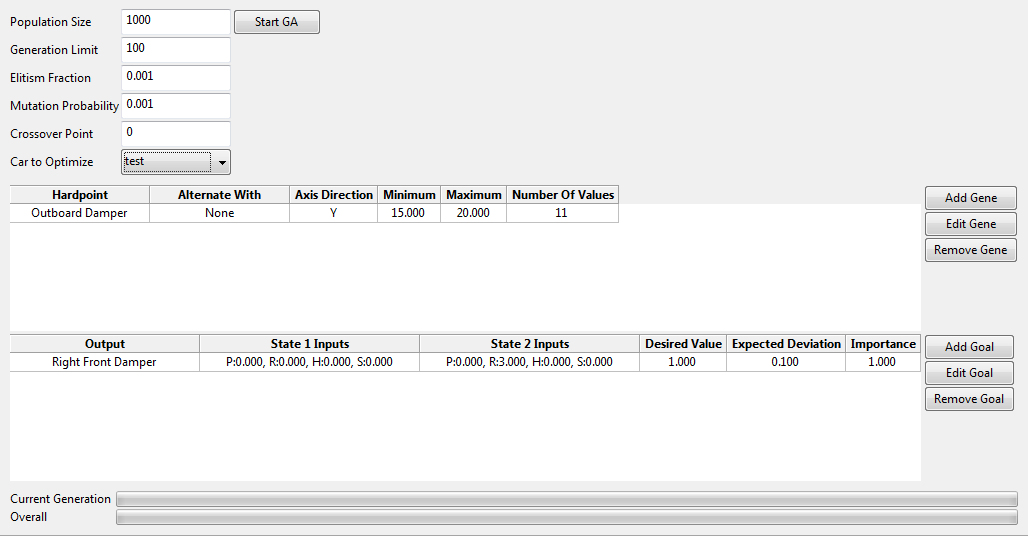
\includegraphics[width=\textwidth]{images/gaPanel}
  \caption{Genetic optimization panel} \label{fig:gaPanel}
  \centering
\end{figure}

There is no \element{Edit Panel} content associated with optimization files.

\section{Genetic Search Algorithms} \label{sec:geneticAlgorithms}

Genetic search algorithms are a stochastic optimization, modeled on the process of evolution and natural selection.  They work by applying a ``survival of the fittest'' approach to optimization problems.  Generally, these algorithms must take the following steps:

\begin{enumerate}
  \item Randomly create initial population
  \item Assign a fitness score to each population member \label{item:assignFitness}
  \item Sort the population according to the fitness score
  \item Breed the members with the highest fitnesses to create the next population \label{item:breed}
  \item Repeat steps~\ref{item:assignFitness}~-~\ref{item:breed} until reaching a predetermined fitness score, number of iterations or other termination criteria
\end{enumerate}

To fit a problem into the required framework, each member must be representable by some type of code. With respect to the optimization, this code must describe the member entirely.  This code is the genotype.  Each code describes a unique representation of the population member.  The representation corresponding to a genotype is a phenotype.

Additionally, a method is required for determining the fitness of each phenotype.  This fitness score must be sortable.

\section{Algorithm Parameters} \label{sec:algorithmParameters}

The interface to the genetic search algorithm implemented in \vvase{} takes several top-level parameters as well as specific parameters for describing the genes and goals.  This section defines the top-level parameters that control the process described in \sref{sec:geneticAlgorithms} above.  Setting the parameter values for specific optimizations takes some trial and error.  The discussion below includes some recommendations and guidelines for setting the parameters, but ultimately the best choices for these parameters are optimization-dependent.

\subsection{Population Size} \label{ssec:populationSize}

The population size is the number of genotypes that are included in the simulation and scoring of each generation.  The population size should be commensurate with the search space.  When there are many possible genes, the population size should be larger.

\subsection{Generation Limit} \label{ssec:generationLimit}

The generation limit sets the run length for the optimization.  The generation limit should be sized proportionally to the number of goals included in the optimization.  It is not uncommon for convergence rates to be slow for the early generations.  If the population size is very large, it is also likely that more generations must be simulated in order to converge successfully.

\subsection{Elitism Fraction} \label{ssec:elitismFraction}

During the breeding process, it is possible that all of the offspring for a given generation fail to achieve a fitness equal to the best fitness from the previous generation.  To guarantee that the best solutions are always carried from one generation to the next (and thus always part of the gene pool), an elitism fraction may be defined.  When the elitism fraction is greater than zero, there will always be at least one genotype carried exactly as-is into the next generation.  When used, it is best to keep the elitism fraction small, however, to ensure that the largest possible number of genotypes are available for the algorithm to use in finding better solutions.

\subsection{Mutation Probability} \label{ssec:mutationProbability}

The mutation probability describes the chance of a single gene being altered during the breeding process.  When a gene is selected for mutation, it is randomly altered such that the result is still within the range of the original gene definition.  Mutation can be used to help broaden the search space, but it tends to slow convergence rates, especially when a high mutation probability is used.  If the mutation probability is increased too much, it is possible that the algorithm will fail to converge at all.

\subsection{Crossover Point} \label{ssec:crossoverPoint}

The crossover point defines the point at which a genotype is split during the breeding process.  For example, if there are four genes, a crossover point of two means the first two genes will come from one parent, where the last two will come from the other.

If the crossover point is set to zero, the selection of genes is randomized.  There is still a guarantee that approximately 50\% of the genes will come from each parent, however it is possible for every other gene to come from the opposte parent, that is, there are no ``blocks'' of genes coming from each parent in the way that a specified crossover point works.

\subsection{Car To Optimize} \label{ssec:carToOptimize}

This drop-down box is used to specify which of the cars the optimization applies.  The original car is not modified; instead a new car is created at the end of the optimization, which represents the solution from the last generation having the best fitness score.

\section{Genes} \label{sec:genes}

The genes define which portions of the car may be modified as part of the search.  The parameters used to identify genes and the values they are allowed to assume are discussed below.  Genes can be added or removed by clicking the \button{Add Gene} and \button{Remove Gene} buttons to the right of the list of genes.  Existing genes can be edited by doubling-clicking an entry in the list of genes or by clicking the \button{Edit Gene} button.

\subsection{Hardpoint} \label{ssec:genesHardpoint}

The hardpoint parameter defines which of the suspension points is the phenotype for this gene.  As the encoding of the gene changes, it is the location of this point that will be modified.

\subsection{Alternate With} \label{ssec:genesAlternateWith}

In some cases it is desirable to lock two hardpoints together such that that share a common coordinate value.  This is sometimes useful for modifying inboard control arm positions, for example; both the forward and rearward points can be modified together.

This parameter is optional.

\subsection{Axis Direction} \label{ssec:genesAxisDirection}

This specifies which of the three ordinate dimensions to vary.  If it is desired for a single hardpoint to be optimized in more than one direction, multiple genes must be defined, each with a different axis direction specified.

\subsection{Minimum} \label{ssec:genesMinimum}

This specifies the minimum allowable value for the phenotype to assume.

\subsection{Maximum} \label{ssec:genesMaximum}

This specifies the maximum allowable value for the phenotype to assume.

\subsection{Number of Values} \label{ssec:genesNumberOfValues}

The number of values defines the granularity of the search space.  The location of the hardpoint will only be able to assume certain finite numbers in the range from minimum to maximum.  Using a large number of values can significantly increase the search space and may require increasing the population size in order to ensure convergence.

\section{Goals} \label{sec:goals}

The goals define which kinematic outputs are targeted in the optimization.  In addition, the fitness function is formulated based on these values.  Goals can be added or removed by clicking the \button{Add Goal} and \button{Remove Goal} buttons to the right of the list of goals.  Existing goals can be edited by doubling-clicking an entry in the list of goals or by clicking the \button{Edit Goal} button.

\subsection{Output} \label{ssec:goalsOutput}

This specifies which kinematic output is targeted.

\subsection{State 1 Inputs} \label{ssec:goalsState1Inputs}

The kinematic inputs are roll, pitch, heave and rack travel.  This is the kinematic state at which the output is evaluated.

\subsection{State 2 Inputs} \label{ssec:goalsState2Inputs}

Optionally, the user may check the option for \button{Optimize difference between states}.  If selected, two text boxes are available for each kinematic input.  The kinematic output will be evaluated at both conditions and the difference between the output at the defined states, rather than the value of the output itself, becomes the target of the optimization.

\subsection{Desired Value/Desired Change} \label{ssec:goalsDesiredValue}

The desired value defines the criteria for the optimization.  If the option for \button{Optimize difference between states} is selected, the criteria becomes the change between the output at the defined states, rather than the value of the output itself.

\subsection{Expected Deviation} \label{ssec:goalsExpectedDeviation}

The expected deviation is the anticipated error between the achieved solution and the desired value or desired change.  This is included as a weighting factor in the fitness function.  It is useful when multiple goals are included in an optimization, and given the input parameters it is easier to achieve a closer fit for one output than another, or alternatively, when one goal has a large value and another has a small value.  Without including the expected deviation, the fitness function may be dominated by a single goal, resulting in other goals being ignored during the optimization.

\subsection{Relative Importance} \label{ssec:goalsRelativeImportance}

The relative importance is a weighting factor included in the fitness function.  Typically the importance values may be set to one, but if certain goals are not being achieved during optimizations, the relative importance can be used to assign more or less weight to certain goals.

\section{Hints} \label{sec:hints}

There is no substitute for experience in creating optimization and observing the results achieved, but without some guidance it can be difficult to get started.  In this section, some additional details on genetic search algorithms are discussed and how they might vary from traditional optimization techniques.  There are also some best practices and guidelines that may be helpful when setting up optimization parameters.

\subsection{Differences from Classical Optimization} \label{ssec:differences}

Genetic search algorithms operate very differently from classical optimizations.  This difference in operation principles is what provides the ability to tackle complex problems, but it can also lead to poor results if the differences are not well understood.

Classical optimizations have a value or a set of values (similar to genes) that are varied in order to attempt to minimize or maximize a fitness function (which could be the same as the fitness function defined by setting optimization goals).  The values are usually altered according to the change in the resulting fitness score.  For example, if the goal is to find the value of $x$ that minimizes $f \left( x \right)$, for some algorithm the sequence might look something like this (assume an initial guess of $x=0$):

\begin{center}
  $x = 0; f \left( x \right) = 10$\\
  $x = 5; f \left( x \right) = 6$\\
  $x = 7; f \left( x \right) = 3$\\
  $x = 9; f \left( x \right) = 4$\\
  $x = 8; f \left( x \right) = 2$
\end{center}

Initially, the algorithm took a relatively large step and guessed five in the second iteration.  The function evaluates to a smaller value, so it keeps going in the direction of increasing $x$.  This works for another iteration, but in the fourth iteration, $f \left( 9 \right)$ evaluates to four, which is greater than the result at $x=7$.  So the algorithm takes a step back and guesses eight, which must have been the right move, since $f \left( 8 \right)$ evaluates to two.  Or maybe not --- what if the global minimum for $f \left( x \right)$ occurs at $x=20$?  Apparently, this algorithm would never reach that point, instead ending the search at a local minimum in the vicinity of $x=8$.  This is a property of many classical optimization algorithms --- they tend to converge at local inflection points instead of guaranteeing a global optimum.

Genetic search algorithms certainly do not guarantee arrival at a global optimum, but they can help to avoid this common trap.  With a sufficiently large population size, genetic search algorithms can cover a broad portion of the solution space, which can provide confidence that a local optimum has been found.  When the solution space has many local inflection points and/or the solution space contains steep gradients, it is often helpful to increase the population size.

Another difference is the way in which the independent variables are represented.  Classical algorithms store these values directly.  Using the above example again, the algorithm tried $x=7$ and then $x=9$, and when the evaluation result increased, the algorithm then tried $x=8$.  A different algorithm might have tried $x=7$, $x=9.5$ and then $x=8.2$.  All of these values of $x$ are real numbers, and therefore they are valid inputs.

Genetic search algorithms work differently --- the allowable input values are defined when the optimization is started.  The algorithm must be told that $x$ is allowed to take on the values of seven, eight and nine.  Or, it is possible that the algorithm was not told it was allowed to choose $x=8$ and it could have returned $x=7$ as the optimal solution.

This might sound undesirable, but it can be a very useful property.  By limiting the resolution of the solution space, the number of possible solutions is reduced from infinity to a finite number.  For solution spaces with smooth changes and a global optimum that is very different from the local optima, larger steps can be used to reduce the computational effort required to converge.  It is an important point, however, since it behaves differently from other algorithms and can lead to unexpected results if it is not considered.

These differences make genetic search algorithms well-suited to solving optimization problems with complex, high-dimensional solution spaces.  These differences also make genetic search algorithms comparatively inefficient for simple optimizations.  In the event that a simple optimization is required, it is beneficial to include only genes that directly affect the goals, use a large number of values that these genes may assume, choose a relatively large population size and choose a low generation limit.

\subsection{Best Practices} \label{ssec:bestPractices}

This section summarizes some genetic optimization best practices.

\begin{description}
\item[Test for Proper Population Size] Too small and the solution may be sub-optimal, too large and CPU cycles are wasted.  A helpful test is to set an artificially low generation limit (maybe just a few generations) and run the optimization several times.  Examine the optimization result.  Do all of the genes have the same phenotype, or is there variation in the results?  If the results are all very similar, it is likely that the solution space is too small for the specified population.  After just a handful of generations, there should be a great deal of variation (for a properly sized population, the phenotypes should be random at this point).  Knowing if the population is too small is more difficult and often required running a full optimization and checking for convergence.
\item[Using Enough Generations] For complex optimizations, be sure to use a generation limit that is high enough to allow the solution to converge.  As a rough starting point, consider using the following expression:  $limit = 10^{number of goals}$.
\item[Start coarse and refine] To reduce computational effort and improve solution speed, start with relatively small numbers of values for each gene.  After narrowing the solution space by running this coarse simulation, update the allowable range of each gene to be smaller, centered around the most recent optimum, keeping the number of values constant.  Of course, if the solution space has steep gradients, it may be required to start with a large, finely distributed solution space from the beginning.
\item[Separate independent optimizations] Genetic search algorithms are helpful for finding solutions to optimization problems that are tightly coupled --- when every gene has some influence over every goal.  If it is desired to optimize two independent goals (for example, front roll center movement and rear roll center movement), it is best to use separate optimizations.
\end{description}
